This section covers the collection of the component models into non-linear state space form, of two vectors containing the state equations and the constraint equations respectively $f(x,u)$ and $ g(x,u) $.

\todo[inline]{Vi bruger egentlig ikke g-matricerne til noget. Måske skal det helt udelades og beholdes på den form det er nu.}

\textbf{NOTE: Currently the constraints of the system (the algebraic equations) are removed from this section because they are too extensive}


In \cref{fig:Block_diagram_inout} the interface variables are split out to show which variables are used as inputs and outputs for each component. Some inputs to components are highlighted in red to signify that they are currently not found as an output of a component. Steady State values (operating points) for these are found from the Hi-Fi simulation. Blue variables are outputs of components which are currently not used by the following component. Each component block also contains the names of the states they contain.

\begin{figure}[h!]
	\centering
	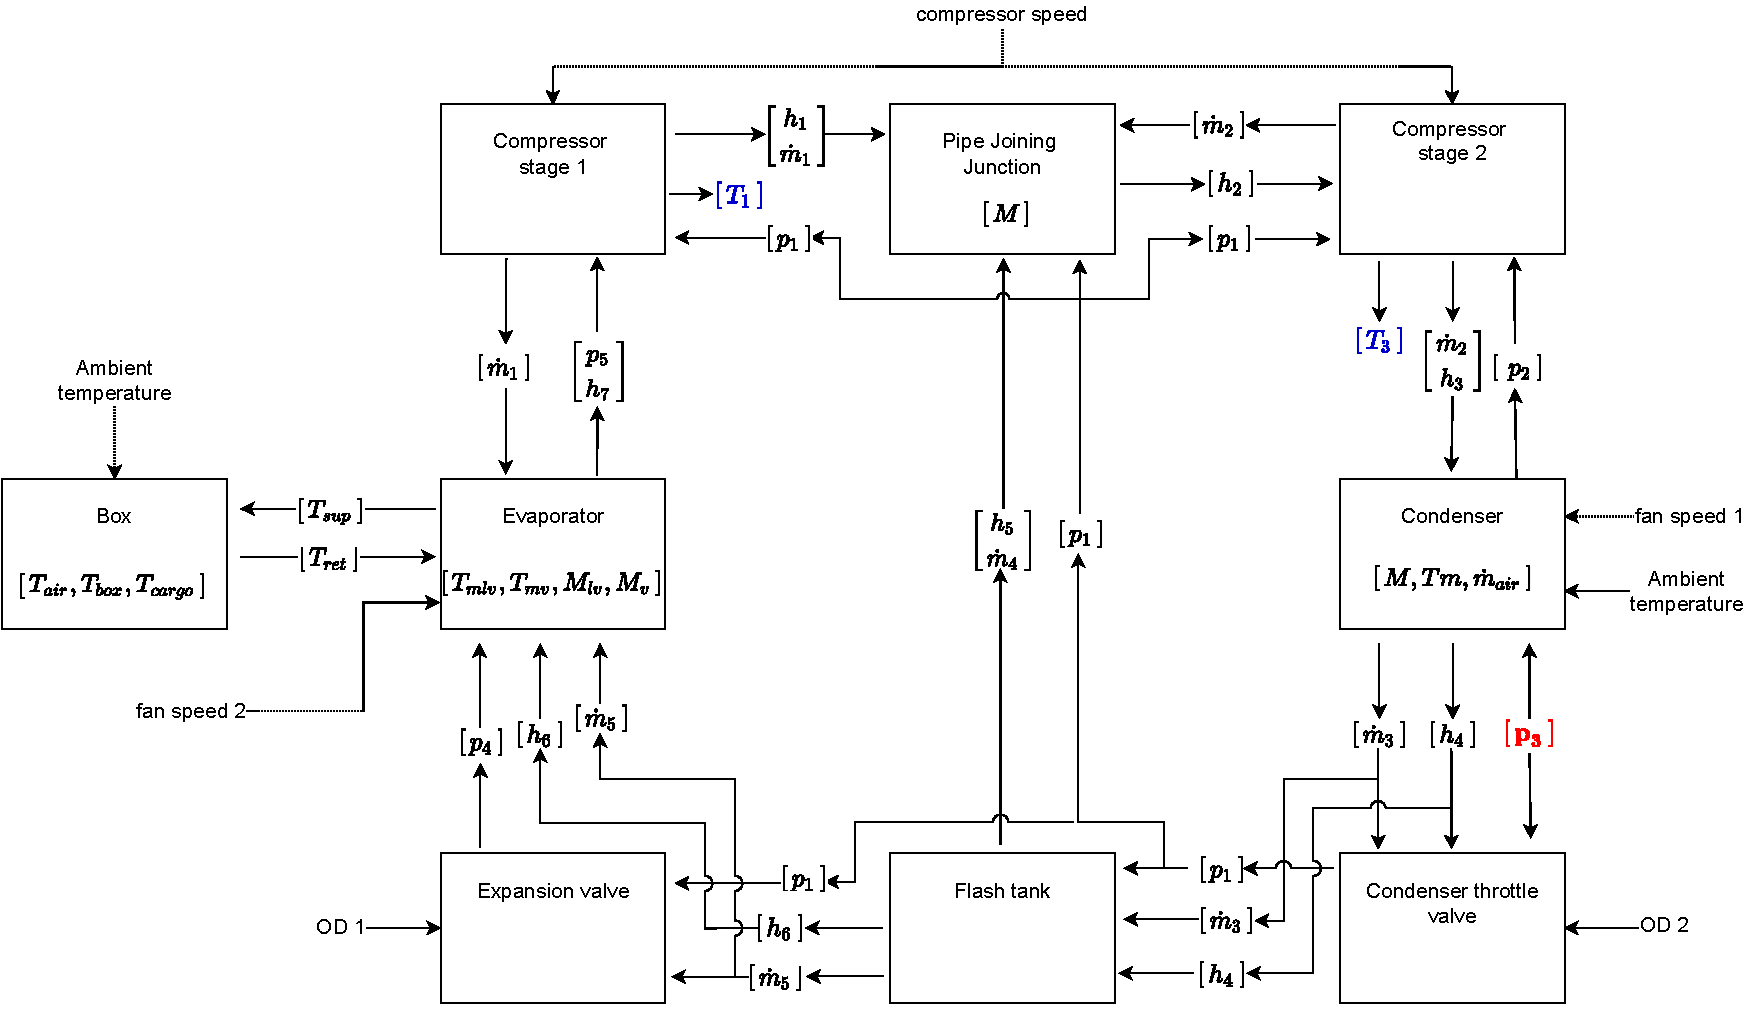
\includegraphics[width=1\textwidth]{Graphics/Block_Diagram_inout.pdf}
	\caption{Block diagram of input/output relationship of interface variables}
	\label{fig:Block_diagram_inout}
\end{figure}


\newpage
\subsubsection{State variables}

Through the component model section the behavior of the system components was described. Due to the large variance in the dynamic speed of the system parameters, the fast variables were defined algebraically, while the slow dynamics were modeled with differential equations. This is possible since the fast variables settle to steady state values without oscillatory behavior. \\

While including the dynamics of the faster parameters would yield a potentially more accurate model, it is unnecessary from a control perspective, as this model is intended for control of the slow dynamics. In addition, the added accuracy will likely be unnoticeable due to various uncertainties in the model. The specific decision of which parameters to model dynamically is heavily inspired by previous work \cite{Sorensen2013}.\\
The parameters described with differential equations are the system states. The differential equations are collected a vector in \cref{eq:f_noSub}.


% F: States
% ------------------------------------

\begin{equation} \label{eq:f_noSub} \renewcommand{\arraystretch}{2.4}
	f(x,u) =  \dfrac{d}{dt} \begin{bmatrix}
		M_{pjj}			\\				%pjj
		M_{con} 		\\				%condenser
		T_m 			\\				%condenser
		\dot{m}_{air}	\\				%evaporator
		T_{mlv}			\\				%evaporator
		T_{mv}			\\				%evaporator
		M_{lv}			\\				%evaporator
		M_v				\\				%evaporator
		T_{air}			\\				%box
		T_{box}			\\				%box
		T_{cargo}		\\				%box

	\end{bmatrix}
	=
	\begin{bmatrix}
		\dot{m}_1 + \dot{m}_4 - \dot{m}_2 \\										%pjj
		\dot{m}_{2} - \dot{m}_{3}	\\												%condenser
		\dfrac{Q_{rm} - Q_{ma}}{M_m \cdot Cp_m} \\									%condenser
		\dfrac{\bar{\dot{m}}_{air}  - \dot{m}_{air}} {10s}		\\					%evaporator
		\dfrac{Q_{aml}-Q_{ml} + Q_{mvml}}{M_m \cdot Cp_m \cdot \sigma}        \\	%evaporator
		\dfrac{Q_{amv} - Q_{mv} - Q_{mvml}}{M_m \cdot Cp_m \cdot (1- \sigma)}	\\	%evaporator
		\dot{m}_{5} - \dot{m}_{dew}		\\											%evaporator
		\dot{m}_{dew} - \dot{m}_{1}	\\												%evaporator
		\dfrac{Q_{ca} + Q_{ba} + Q_{fan} -Q_{cool}}{M_{air} \cdot Cp_{air}} \\		%box
		\dfrac{Q_{amb} - Q_{ba}}{M_{box} \cdot Cp_{box}} \\							%box
		\dfrac{-Q_{ca}}{M_{cargo} \cdot Cp_{cargo}}									%box
	\end{bmatrix}
\end{equation}


Most variables in \cref{eq:f_noSub} are substituted with the algebraic equations defined for the different model components. As such the states, inputs and disturbances are included in the state derivatives. The function $f(x,u)$ is thus the nonlinear model of the system. It contains 11 states, 5 control inputs and 1 disturbance.

The control inputs are:

\begin{center}
	\begin{tabular}{l p{10cm}}
		$ \Theta_1 $  & The valve opening degree of the \\
		$ \Theta_2 $  & The valve opening degree of the \\
		$ U_{fan_1} $ & The condenser fan speed         \\
		$ U_{fan_2} $ & The evaporator fan speed        \\
		$ \omega $    & The compressor speed
	\end{tabular}
\end{center}

The disturbance is:

\begin{center}
	\begin{tabular}{l p{10cm}}
		$ T_{ambi} $  & The ambient air temperature
	\end{tabular}
\end{center}